To understand the specific characteristics of PaaS-hosted web APIs and the potential
of this restricted domain to facilitate efficient static analysis, 
we next statically analyze 35 real world App Engine web APIs (taken from public 
repositories). These web APIs are open 
source and written in Java and run over Google App Engine or AppScale without modification.
We plan to make these applications publicly available upon publication.
We analyze these web APIs 
using the Soot framework~\cite{Vallee-Rai:2010:SJB:1925805.1925818} 
and present characteristics that have influenced our design for Cerebro.

\begin{figure}
\centering
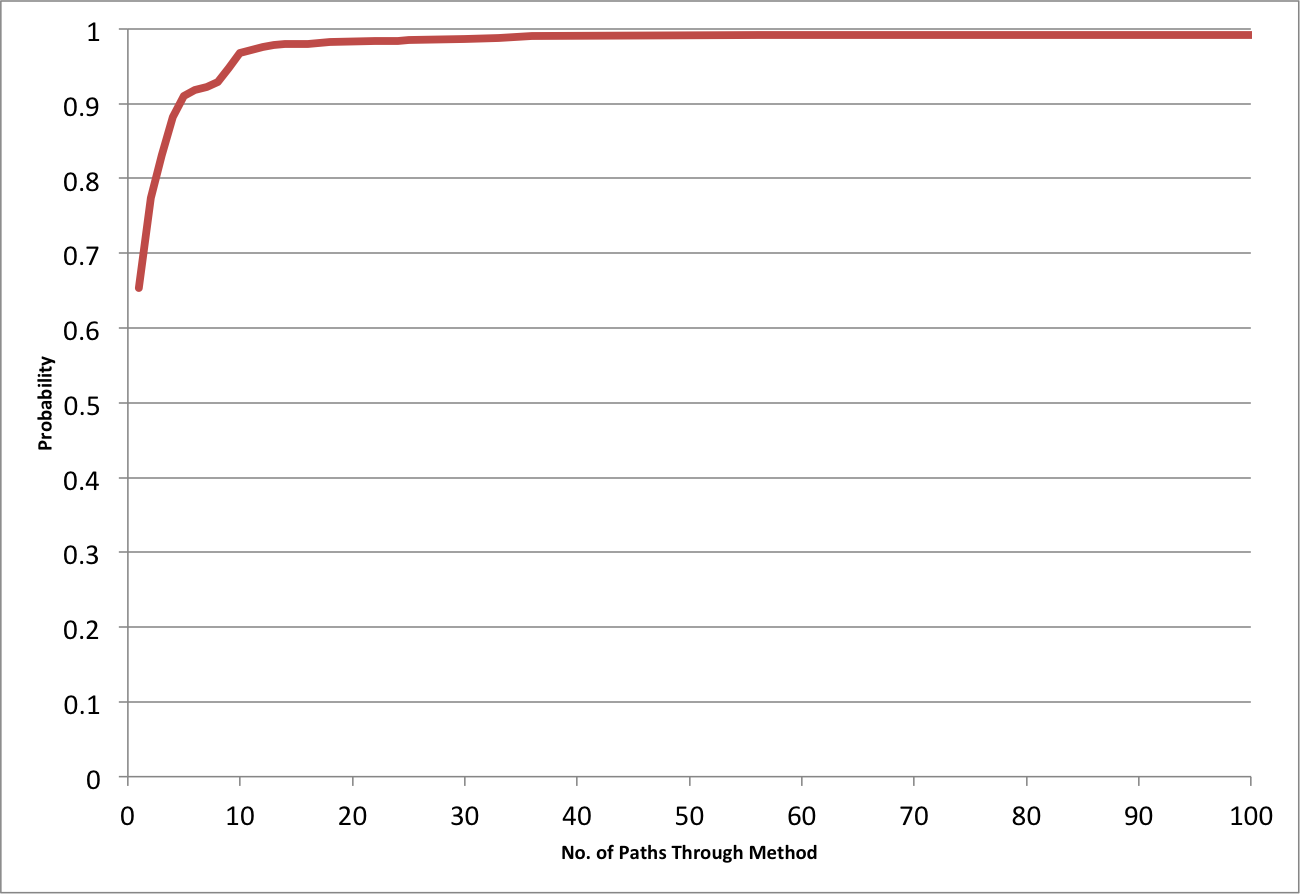
\includegraphics[scale=0.35]{path_count_cdf}
\caption{CDF of the number of static paths through methods in the surveyed web APIs.}
\label{fig:path_count_cdf}
\end{figure}

There is a total of 1458 methods (API operations) in this set of web APIs.
Figure~\ref{fig:path_count_cdf} shows the cumulative distribution of 
static program paths in these methods.
Approximately 97\% of the methods considered in the analysis have 10 or fewer paths. 
Moreover,  99\% of 
the methods have 36 or fewer paths. However, the CDF is heavy tailed
(truncated at 100 but grows to 34992). As such, a small number of methods 
contain very large numbers of paths.
Fortunately, over
65\% have exactly 1 path (i.e. there are no branches).

Next we consider the looping behavior of web APIs. 
1286 of the methods (88\%)
considered in the study
do not have any loops. 172 methods (12\%) contain loops. 
We believe that this characteristic is due to the fact that 
the PaaS SDK and the platform restrictions (quotas) discourages 
looping.

Moreover, approximately 29\% of all the loops in 
the analyzed code do not contain any cloud SDK invocations. 
A large majority of the loops (61\%) that methods do contain are
used to iterate over a dataset that is returned from the datastore cloud SDK interface 
of App Engine (i.e iterating on the result set 
returned by a datastore query). We refer to this particular type of 
loop as \textit{iterative datastore reads}. 
We use these heuristics when designing the loop handling capability of Cerebro.

\begin{table}[htdp]
\caption{Number of times different cloud SDK interfaces are called in web applications.}
\begin{center}
\begin{tabular}{|c|c|}
\hline
Cloud SDK Interface & No. of Invocations \\ \hline
blobstore & 7 \\ \hline
channel & 1 \\ \hline
datastore & 735 \\ \hline
files & 4 \\ \hline
images & 3 \\ \hline
memcache & 12 \\ \hline
search & 6 \\ \hline
taskqueue & 24 \\ \hline
tools & 2 \\ \hline
urlfetch & 8 \\ \hline
users & 44 \\ \hline
xmpp & 3 \\ \hline
\end{tabular}
\end{center}
\label{tab:sdk_call_counts}
\end{table}

Table~\ref{tab:sdk_call_counts} lists the number of times each cloud 
SDK interface has been called in the sample of
35 web applications. The Datastore API is the most commonly used interface 
by these App Engine applications.
This is because data storage and access is a fundamental 
capability required by most web APIs and the PaaS
disallows local filesystem
access for scalability and portability (relocatability) reasons.

\begin{figure}
\centering
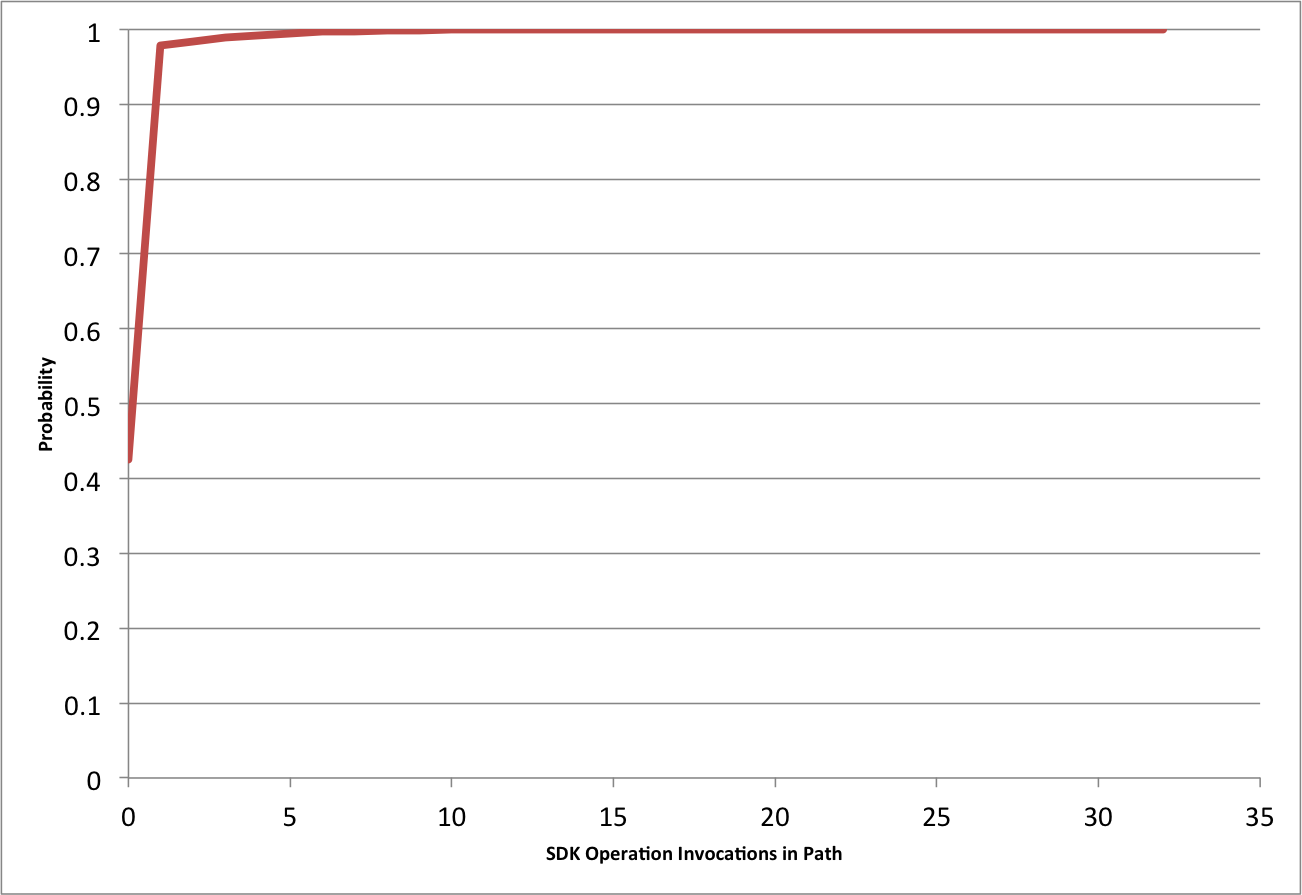
\includegraphics[scale=0.35]{sdk_call_count_cdf}
\caption{CDF of cloud SDK call counts in paths of execution.}
\label{fig:sdk_call_count_cdf}
\end{figure}

Next, we explore the number of cloud SDK calls made along 
different paths of execution in the web APIs. For this study
we consider all paths of execution through the methods (64780 total paths). 
Figure~\ref{fig:sdk_call_count_cdf}
shows the cumulative distribution of the number of SDK calls within paths.
Approximately 98\% of the paths have 0 or 1 cloud SDK calls. 
The probability of finding an execution path with more than
5 cloud SDK calls is smaller than 1\%.
This implies in most cases Cerebro will likely be able to make response 
time predictions by analyzing the
historical performance data of a very small number of cloud SDK operations.

Finally, our experience with App Engine web APIs indicates that a significant
portion of the total time of a method (web API operation) is spent in cloud SDK calls.
Confirming this hypothesis requires careful instrumentation (i.e. difficult
to automate) of the web API codes.  We performed a small number of experiments 
which support this claim.  We therefore assume this to be the case for all
App Engine web APIs and thus focus our static analysis on estimating the 
worst case execution time of an API from its cloud SDK operations.
In the next section, we describe our design and implementation of Cerebro
that takes advantage of these characteristics and assumptions and then
use this prototype to evaluate the accuracy of our predictions as an indicator
of whether this assumption holds.
